%-------------------------------------------------------------
% DESCOMPOSICIÓN 3+1
%-------------------------------------------------------------

Las ecuaciones de campo de Einstein (\ref{eq:Einstein}) para la gravedad est\'{a}n escritas de manera covariante, por lo que tiempo y espacio son tratados en igualdad de condiciones. Sin embargo, para estudiar la gravedad como una teor\'{i}a de campo y definir una formulaci\'{o}n Hamiltoniana, donde el espacio evolucione en el tiempo se debe romper la covariancia. Una técnica para hacer dicha descomposici\'{o}n es el formalismo ADM o descomposici\'{o}n (3+1) de Relatividad General.

\subsection{Formalismo ADM o descomposici\'{o}n (3+1)}
\label{subsec:3+1}

La descomposici\'{o}n (3+1) consiste en hacer una foliaci\'{o}n del espacio-tiempo con una familia de hipersuperficies espacialoides, cada una definiendo un instante de tiempo (figura \ref{fig:Foliation}). Para realizar la foliaci\'{o}n, se considera que el espacio-tiempo de inter\'{e}s es globalmente hiperb\'{o}lico, esto es que tienen una superficie de Cauchy. Se puede identificar la foliaci\'{o}n con el conjunto de superficies de nivel de un campo escalar $t(x^{\alpha})$ ($t = constante$), correspondientes a una familia de hipersuperficies espacialoides, que ser\'{a}n denotadas por $\Sigma_{t}$. Esta funci\'{o}n de tiempo es completamente arbitraria; salvo porque $t$ sea simplemente valuada de $x^{\alpha}$, y $n_{\alpha} \propto \partial_{\alpha} t$, el normal unitario a la hipersuperficie $\Sigma_{t}$, sea un campo vectorial tipo tiempo con direcci\'{o}n al futuro.

\begin{figure}[H]
\label{fig:Foliation}
\centering
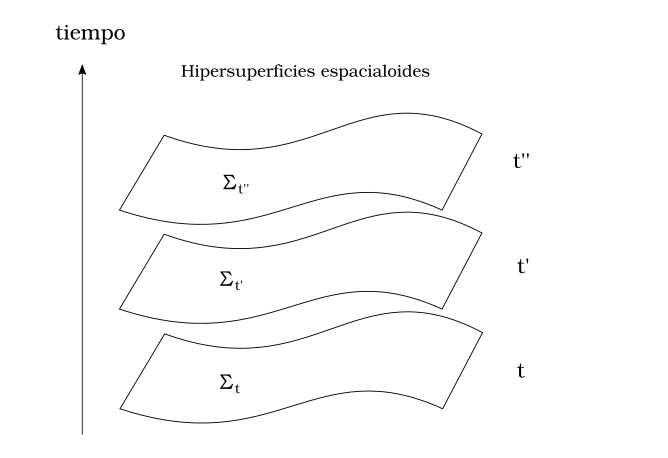
\includegraphics[width=0.7\textwidth]{Foliation.png}
\caption{Foliaci\'{o}n del espacio-tiempo en hipersuperficies espacialoides.}
\end{figure}

En cada hipersuperficie $\Sigma_{t}$ se usar\'{a}n las coordenadas $y^{a}$, que se relacionar\'{a}n mediante una congruencia de curvas $\gamma$ parametrizadas por la funci\'{o}n de tiempo $t$ y vector tangente (tipo tiempo) $t^{\alpha} = d x^{\alpha} / d t$ a la curva. Estas curvas intersectan a las hipersuperficies $\Sigma_{t}$, pero no necesariamente de manera ortogonal ni tampoco se debe asumir que son geod\'{e}sicas. 

Una curva en particular $\gamma_{q}$ de la congruencia, define un mapeo de un punto $q$ en $\Sigma_{t}$ a un punto $q'$ en $\Sigma_{t'}$, y tambi\'{e}n a un punto $q''$ en $\Sigma_{t''}$, y as\'{i} sucesivamente (figura \ref{fig:curvagamma}). Para fijar las coordenadas de $q'$ y $q''$, dadas las coordenadas $y^{a}(q)$ en $\Sigma_{t}$, simplemente se impone que $y^{a}(q) = y^{a}(q') = y^{a}(q'')$. De esta manera, $y^{a}$ se mantiene constante sobre cada una de las curvas $\gamma$.

\begin{figure}[H]
\label{fig:curvagamma}
\centering
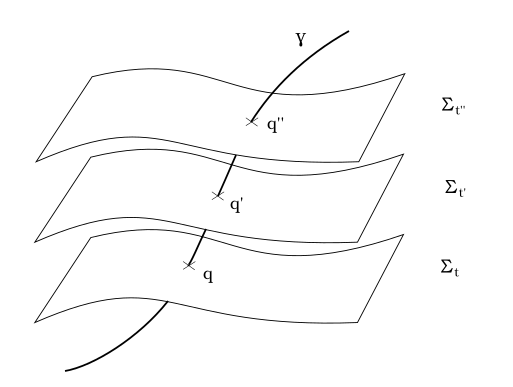
\includegraphics[width=0.5\textwidth]{Gammaintersectingqpoints.png}
\caption{Curva $\gamma$ relacionando puntos de distintas hipersuperficies.}
\end{figure}

N\'{o}tese que por construcci\'{o}n se defini\'{o} un sistema coordenado $(t, y^{a})$ en $\Omega$. As\'{i} que existe una transformaci\'{o}n entre \'{e}ste y el sistema coordenado $x^{\alpha}$, lo que permite expresar las coordenadas originales en t\'{e}rminos de las nuevas, esto es: $x^{\alpha} = x^{\alpha} (t, y^{\alpha})$. Entonces,
%
\begin{align}
\label{eq:dxalpha}
dx^{\alpha} & = \left( \frac{\partial x^{\alpha}}{\partial t} \right)_{y^{a}} dt + \left( \frac{\partial x^{\alpha}}{\partial y^{a}} \right)_{t} dy^{a} \nonumber \\
& = t^{\alpha} dt + e^{\alpha}_{a} dy^{a},
\end{align}
%
donde $t^{\alpha}=\partial x^{\alpha}/\partial t$ es el vector tangente a $\gamma$ y $e^{\alpha}_{a}=\partial x^{\alpha}/\partial y^{a}$ son los vectores tangentes a $\Sigma_{t}$.

El vector tangente $t^{\alpha}$ a la curva $\gamma$ en general no es ortogonal a $\Sigma_{t}$ (i.e., no es paralelo al vector normal $n^{\alpha}$). Ahora bien, el normal unitario es $n_{\alpha} = -N \partial_{\alpha} t$, donde $N$ es conocida como la \emph{funci\'{o}n de lapso} que se encarga de normalizar, as\'{i} que $N$ es la proyecci\'{o}n de $t^{\alpha}$ sobre el normal unitario\footnotemark. Tambi\'{e}n n\'{o}tese que $t^{\alpha}$ va a tener una proyecci\'{o}n sobre los vectores tangentes $e^{\alpha}_{a}$, estas proyecciones forman un vector tipo espacio $N^{a}$ tangente a $\Sigma_{t}$ y conocido como \emph{vector de corrimiento}.
\footnotetext{Ya que $t^{\alpha} \partial_{\alpha} t = 1$.}

\begin{center}
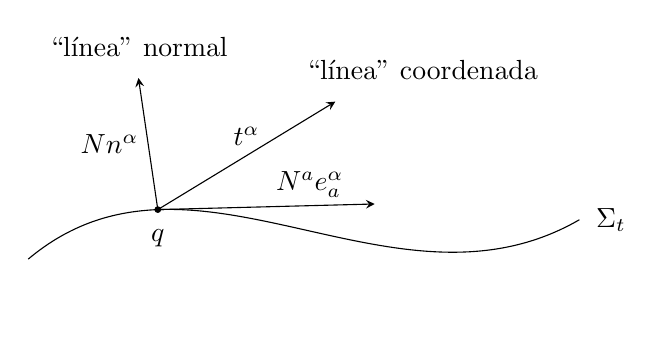
\begin{tikzpicture}
%
\draw (-3.5, 0) to[out=40,in=-150] 
  coordinate[pos=0.25] (aux1)(3.5, 0.5);
%
\draw[fill] (aux1) circle (1pt);
\node[label=below:$q$] at (aux1) {};
%
\coordinate (aux2) at (-2.1,2.3); 
\coordinate (aux3) at (0.9,0.7);
%\draw (aux1) ->  node [left] {$N n^{\alpha}$} (aux2);
%\draw (aux1) ->  node [above] {$N^{a} e^{\alpha}_{a}$} (aux3);
\path[->,>=stealth] (aux1) edge node [left] {$N n^{\alpha}$} (aux2);
\path[->,>=stealth] (aux1) edge node [above right] {$N^{a} e^{\alpha}_{a}$} (aux3);
%
\coordinate (aux4) at (0.4,2);
%\draw (aux1) ->  node [above] {$t^{\alpha}$} (aux4);
\path[->,>=stealth] (aux1) edge node [above] {$t^{\alpha}$} (aux4);
%
\node at (3.9, 0.5) {$\Sigma_{t}$};
\node at (-2.1, 2.7) {``l\'{i}nea'' normal};
\node at (1.5,2.4) {``l\'{i}nea'' coordenada};
%
\end{tikzpicture}
\end{center}

As\'{i}, el vector $t^{\alpha}$ se descompone como,
%
\begin{equation}
\label{eq:descompt}
t^{\alpha} = N n^{\alpha} + N^{a} e^{\alpha}_{a}.
\end{equation}

Sustituyendo \eqref{eq:descompt} en \eqref{eq:dxalpha} y tomando en cuenta que el elemento de l\'{i}nea est\'{a} dado por $ds^{2} = g_{\mu \nu} d x^{\mu} d x^{\nu}$, se sigue que en el nuevo sistema coordenado
%
\begin{equation}
\label{eq:dslapseandshift}
ds^{2} = (-N^{2} + N_{a} N^{a}) dt^{2} + 2 N_{a} dt dy^{a} + h_{ab} dy^{a} dy^{b}.
\end{equation}

%La ecuaci\'{o}n \eqref{eq:dslapseandshift} es la descomposici\'{o}n (3+1) de la m\'{e}trica. Expl\'{i}citamente se tiene
%
%\begin{equation}
%\label{eq:metric31}
%g_{AB} =
 %\begin{pmatrix}
 %-N^{2} + N_{a} N^{a} & N_{a} \\
 %N_{b} & h_{ab}
 %\end{pmatrix},
%\end{equation}
%
%\begin{equation}
%\label{eq:invmetric31}
%g^{AB} =
%\begin{pmatrix}
 %-1 / N^{2} & N^{a} / N^{2} \\
 %N^{b} / N^{2} & h^{ab} - N^{a} N^{b} / N^{2}
 %\end{pmatrix}.
%\end{equation}

Vale la pena recordar que $h_{ab}$ es la m\'{e}trica en $\Sigma_{t}$

Se puede mostrar que
%
\begin{equation}
\label{eq:elemntvol31}
\sqrt{-g} = N \sqrt{h}.
\end{equation}

Las ecuaciones \eqref{eq:descompt}, \eqref{eq:dslapseandshift} y \eqref{eq:elemntvol31} son los resultados fundamentales de la descomposici\'{o}n (3+1).